% Created 2023-10-13 Fri 10:45
% Intended LaTeX compiler: xelatex
\documentclass[aspectratio=1610,xcolor={dvipsnames},hyperref={colorlinks,unicode,linkcolor=violet,anchorcolor=BlueViolet,citecolor=YellowOrange,filecolor=black,urlcolor=Aquamarine}]{beamer}
\usepackage{graphicx}
\usepackage{grffile}
\usepackage{longtable}
\usepackage{booktabs}
\usepackage{wrapfig}
\usepackage{rotating}
\usepackage[normalem]{ulem}
\usepackage{amsmath}
\usepackage{textcomp}
\usepackage{amssymb}
\usepackage{capt-of}
\usepackage{nicefrac}
\usepackage[dvipsnames]{xcolor}
\usepackage[colorlinks,unicode,linkcolor=violet,anchorcolor=BlueViolet,citecolor=YellowOrange,filecolor=black,urlcolor=Aquamarine]{hyperref}
\AtBeginSubsection[]{\begin{frame}<beamer>\frametitle{Section}\tableofcontents[currentsection,currentsubsection]\end{frame}}
\synctex=1
\usepackage{etoolbox}
\useoutertheme{infolines}
\setbeamertemplate{frametitle}{%
\usebeamerfont{frametitle}\insertframetitle\strut%
\vskip-0\baselineskip%
\leaders\vrule width .95\paperwidth\vskip1pt%
\vskip0pt%
\nointerlineskip%
}

%% T for footer
\setbeamercolor{footlinecolor}{fg=cyan,bg=green}
\setbeamercolor{author in head/foot}{fg=blue}
\setbeamertemplate{footline}{%
\leavevmode%
\hbox{%
\begin{beamercolorbox}[wd=.26\paperwidth,ht=2.25ex,dp=1ex,left]{author in head/foot}%
\hspace*{2ex}\usebeamerfont{author in head/foot} Dept. CSE, UT Arlington
\end{beamercolorbox}%
\begin{beamercolorbox}[wd=.50\paperwidth,ht=2.25ex,dp=1ex,center]{author in head/foot}%
\usebeamerfont{title in head/foot}Scalable Modeling \& Imaging \& Learning Lab (SMILE)
\end{beamercolorbox}%
\begin{beamercolorbox}[wd=.24\paperwidth,ht=2.25ex,dp=1ex,right]{date in head/foot}%
\usebeamerfont{date in head/foot}
\insertshortdate{}\hspace*{1em}  % date
\insertframenumber/\inserttotalframenumber\hspace*{2ex}
\end{beamercolorbox}}%
\vskip0pt%
}
\setbeamerfont{footnote}{size=\tiny}
\usepackage{minted}
\setbeamerfont{caption}{size=\scriptsize}
\usetheme{default}
\usefonttheme{serif}
\useinnertheme{circles}
\author{Nasy}
\date{Jul 16, 2023}
\title{LLM as Optimizers and Meta Optimizers}
\hypersetup{
 pdfauthor={Nasy},
 pdftitle={LLM as Optimizers and Meta Optimizers},
 pdfkeywords={},
 pdfsubject={},
 pdfcreator={Emacs 29.0.50 (Org mode 9.5.5)}, 
 pdflang={English}}
\usepackage{biblatex}
\addbibresource{/Users/Nasy/.emacs.d/萚兮/時/refs/ref.bib}
\begin{document}

\maketitle
\begin{frame}{Outline}
\setcounter{tocdepth}{1}
\tableofcontents
\end{frame}

\setcounter{tocdepth}{2}
\section{Large Language Model as Optimizers}
\label{sec:org579998a}

\subsection{Introduction}
\label{sec:orgb8ef026}

\begin{frame}[label={sec:orge2c77d7}]{Introduction}
\begin{itemize}
\item What is LLM as Optimizers?
\begin{itemize}
\item Optimization by PROmpting (OPRO)
\item The goal is to find instructions that maximize the task accuracy.
\end{itemize}
\item With a variety of LLMs, we demonstrate that the best prompts optimized by OPRO outperform human-designed prompts by up to 8\% on GSM8K, and by up to 50\% on Big-Bench Hard tasks.
\end{itemize}
\end{frame}
\subsection{Optimization by PROmpting (OPRO)}
\label{sec:org639c87e}

\begin{frame}[label={sec:org4cabf1a}]{Optimization by PROmpting (OPRO)}
\begin{center}
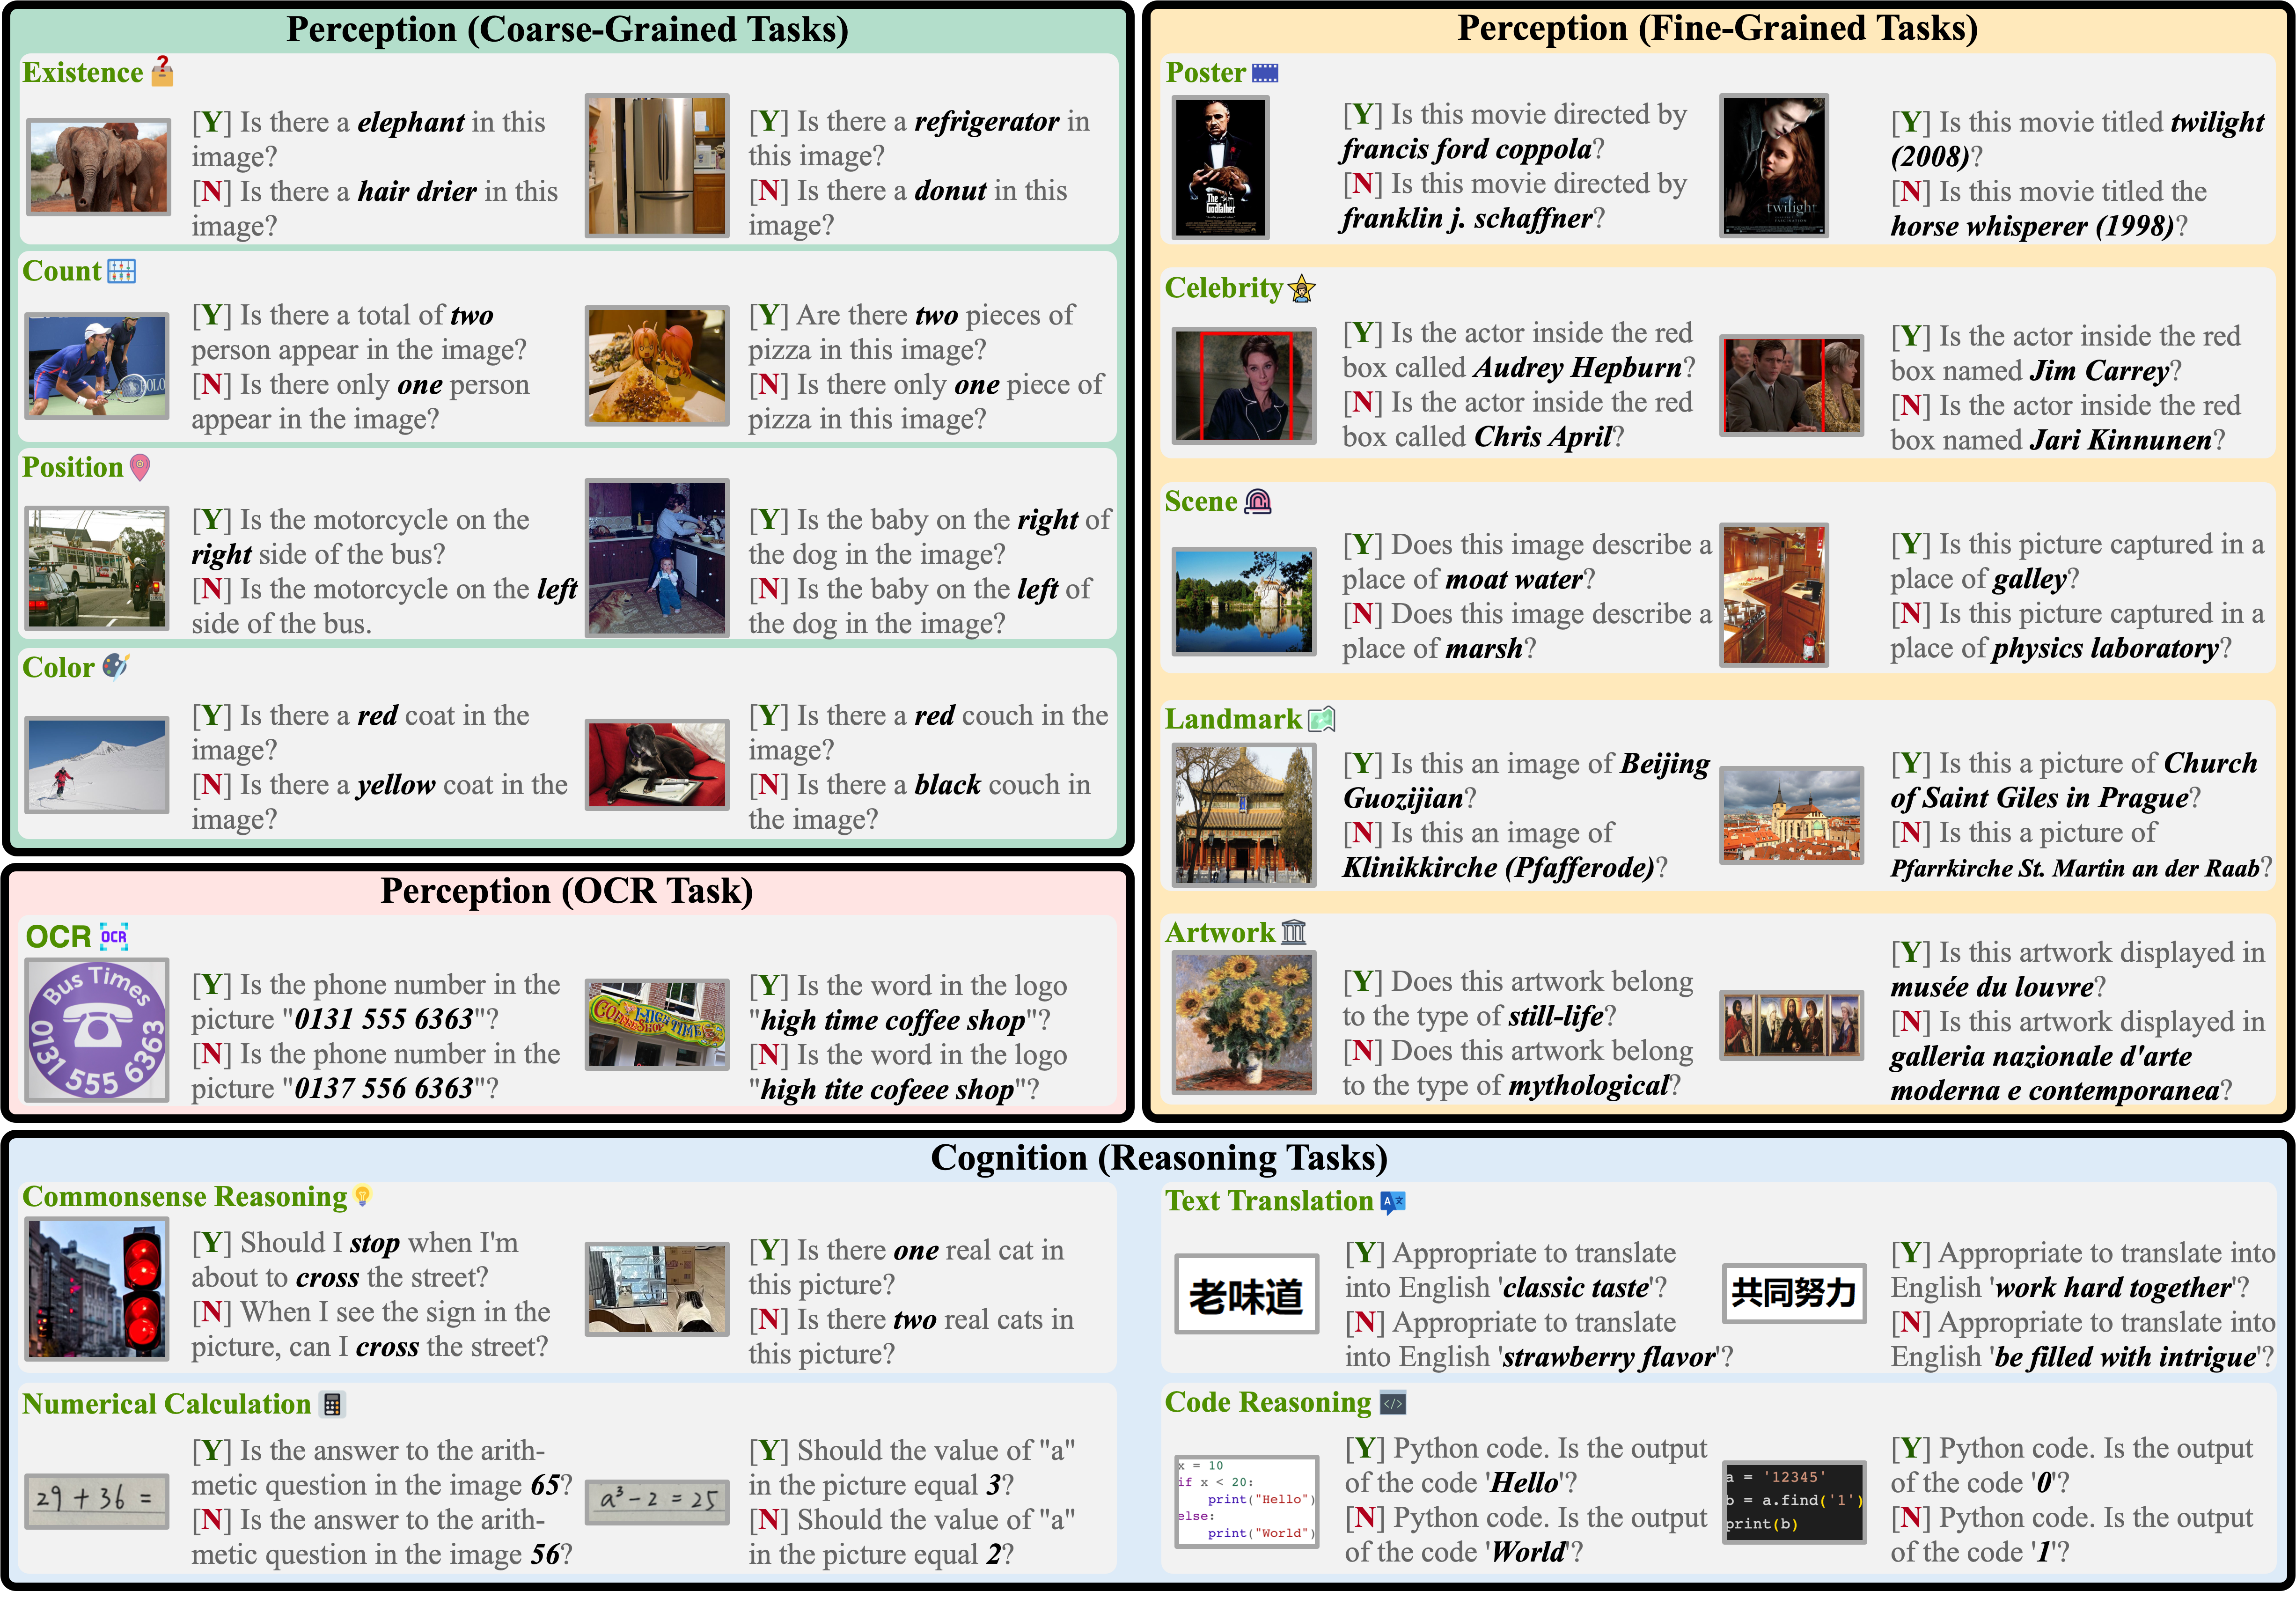
\includegraphics[height=8cm]{./p1.png}
\end{center}
\end{frame}
\begin{frame}[label={sec:org18277b0}]{Example}
\begin{center}
\includegraphics[height=8cm]{./p2.png}
\end{center}
\end{frame}
\begin{frame}[label={sec:org62ba67a}]{Motivation}
\begin{itemize}
\item Making use of natural language descriptions
\begin{itemize}
\item The main advantage of LLMs for optimization is their ability of understanding natural language, which allows people to describe their optimization tasks without formal specifications.
\end{itemize}
\item Trading off exploration and exploitation
\begin{itemize}
\item LLM should be able to exploit promising areas of the search space where good solutions are already found, while also exploring new regions of the search space so as to not miss potentially better solutions.
\end{itemize}
\end{itemize}
\end{frame}
\begin{frame}[label={sec:org2421be3}]{Meta-Prompt Design}
\begin{itemize}
\item Optimization problem description
\begin{itemize}
\item e.g., generate a new instruction that achieves a higher accuracy
\item e.g., the instruction should be concise and generally applicable
\end{itemize}
\item Optimization trajectory
\begin{itemize}
\item The optimization trajectory includes past solutions paired with their optimization scores, sorted in the \alert{ascending} order.
\end{itemize}
\end{itemize}
\end{frame}
\begin{frame}[label={sec:orga371058}]{Solution Generation}
\begin{itemize}
\item Optimization stability.
\begin{itemize}
\item Prompt the LLM to generate multiple solutions at each optimization step, allowing the LLM to simultaneously explore multiple possibilities and quickly discover promising directions to move forward.
\end{itemize}
\item Exploration-exploitation trade-off
\begin{itemize}
\item Tune the LLM sampling temperature to balance between exploration and exploitation. A lower temperature encourages the LLM to exploit the solution space around the previously found solutions and make small adaptations, while a high temperature allows the LLM to more aggressively explore solutions that can be notably different.
\end{itemize}
\end{itemize}
\end{frame}
\subsection{Mathematical Optimization}
\label{sec:org4a75fc6}

\begin{frame}[label={sec:org6894215}]{Mathematical Optimization}
\begin{center}
\includegraphics[width=13cm]{./p3.png}
\end{center}
\end{frame}
\begin{frame}[label={sec:orgd5d5869}]{Mathematical Optimization}
\begin{center}
\includegraphics[width=13cm]{./p4.png}
\end{center}
\end{frame}
\begin{frame}[label={sec:orgd30705c}]{Limitations}
Limitations. We would like to note that OPRO is designed for neither outperforming the stateof-the-art gradient-based optimization algorithms for continuous mathematical optimization, nor
surpassing the performance of specialized solvers for classical combinatorial optimization problems
such as TSP. Instead, the goal is to demonstrate that LLMs are able to optimize different kinds
of objective functions simply through prompting, and reach the global optimum for some smallscale problems.
\end{frame}
\subsection{Prompt Optimization}
\label{sec:org928cf3d}

\begin{frame}[label={sec:org34b61c0}]{Prompt Optimization}
\begin{center}
\includegraphics[height=8cm]{./p5.png}
\end{center}
\end{frame}
\begin{frame}[label={sec:org6a71f6a}]{Prompt Optimization Design}
\begin{itemize}
\item Optimization problem examples.
\item Optimization trajectory
\item Meta-instructions
\end{itemize}
\end{frame}
\begin{frame}[label={sec:orgce30a87}]{Results}
\begin{center}
\includegraphics[height=3.5cm]{./p6.png}
\end{center}

\begin{center}
\includegraphics[height=3.5cm]{./p7.png}
\end{center}
\end{frame}
\begin{frame}[label={sec:org235868d}]{Results}
\begin{center}
\includegraphics[height=8cm]{./p8.png}
\end{center}
\end{frame}
\begin{frame}[label={sec:org4392767}]{Results BBH}
See paper p15.
\end{frame}
\begin{frame}[label={sec:org1af3f91}]{Suggestions}
\url{https://github.com/AGI-Edgerunners/LLM-Optimizers-Papers}
\end{frame}
\section{Conclusion}
\label{sec:orge21aa08}

\begin{frame}[label={sec:orgaeb87e2}]{Conclusion}
\begin{itemize}
\item Optimization by PROmpting (OPRO)
\begin{itemize}
\item The goal is to find instructions that maximize the task accuracy.
\end{itemize}
\item Motivation
\begin{itemize}
\item Making use of natural language descriptions
\item Trading off exploration and exploitation
\end{itemize}
\item Design
\begin{itemize}
\item Optimization problem description
\item Optimization trajectory
\item Meta-instructions
\end{itemize}
\item Results
\end{itemize}
\end{frame}
\section{Uncovering mesa-optimization algorithms in Transformers}
\label{sec:orgc0843ca}

\begin{frame}[label={sec:orgb5bb6c0}]{Introduction}
\begin{itemize}
\item Why?
\begin{itemize}
\item Transformers have become the dominant model in deep learning, but the reason for their superior performance is poorly understood
\end{itemize}
\item How?
\begin{itemize}
\item By reverse engineering a series of autoregressive Transformers trained on simple sequence modeling tasks, the authors reveal the gradient-based mesa-optimization algorithm that drives prediction generation.
\end{itemize}
\item New?
\begin{itemize}
\item Propose a novel self-attention layer, the mesa-layer, that explicitly and efficiently solves optimization problems specified in context
\end{itemize}
\end{itemize}
\end{frame}
\begin{frame}[label={sec:orged38c7b}]{Mesa-Optimization}
\begin{center}
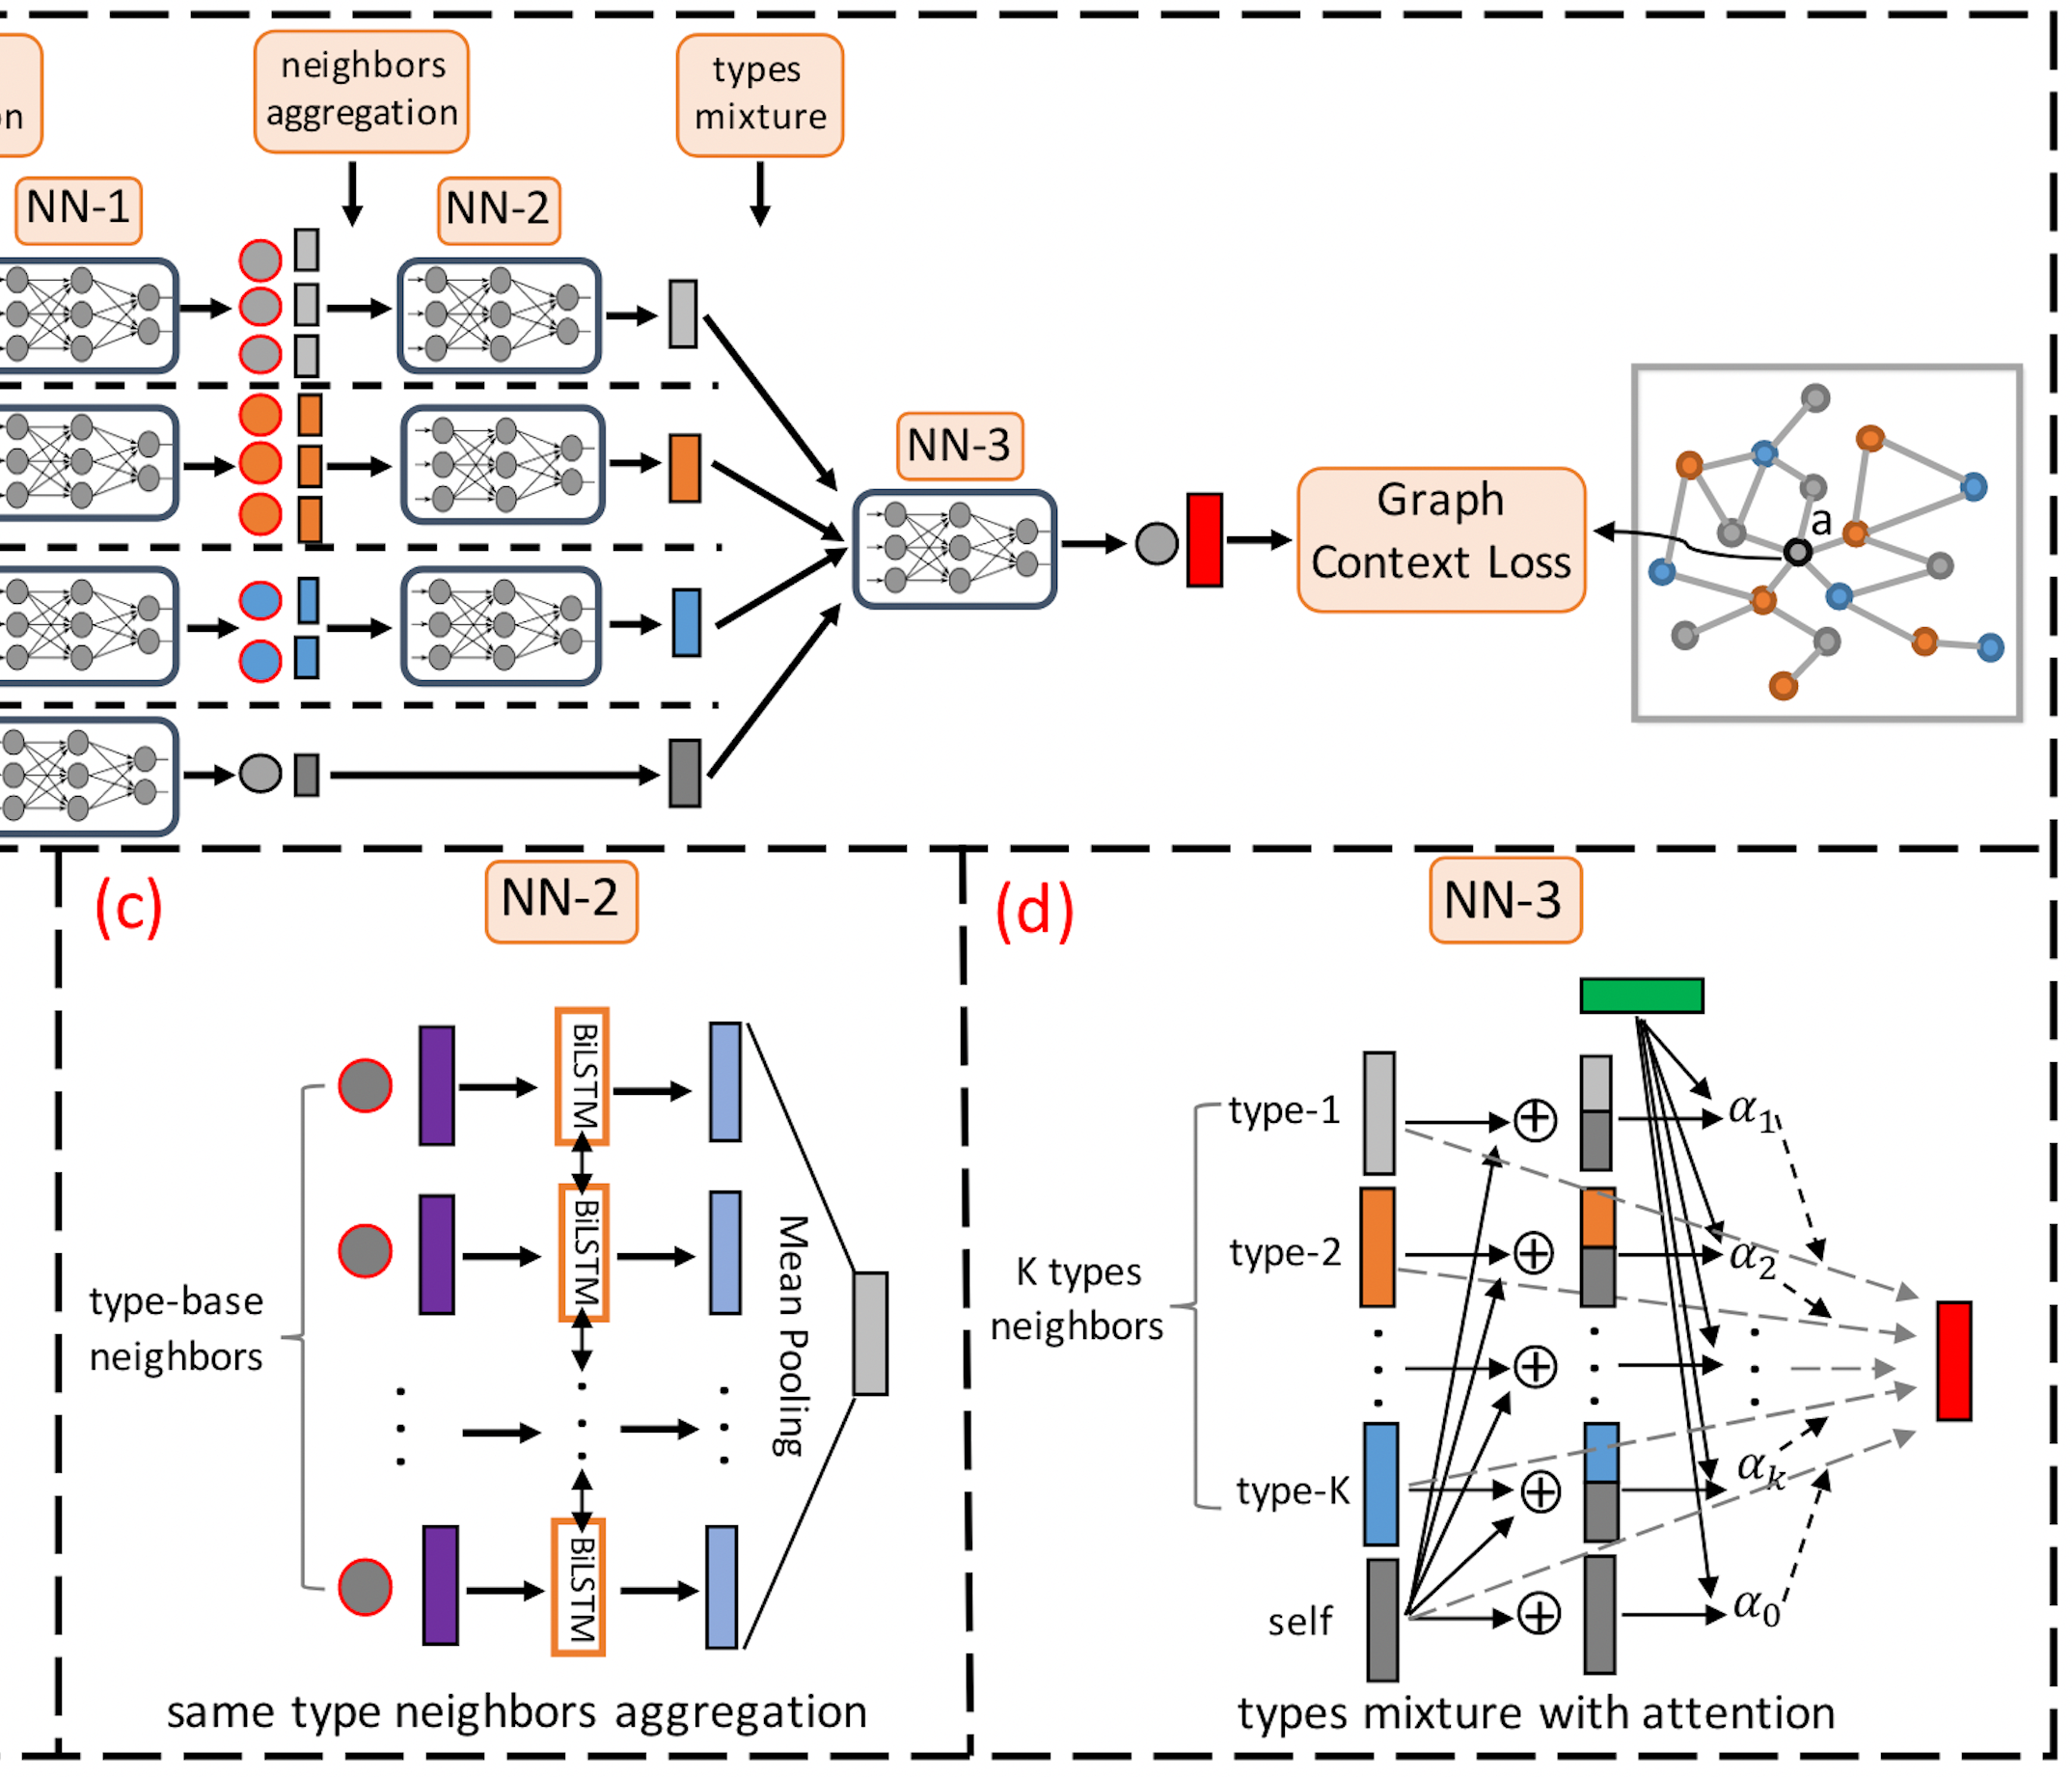
\includegraphics[width=13cm]{./p9.png}
\end{center}
\end{frame}
\begin{frame}[label={sec:orgd6b84c7}]{Mesa-Optimization}
\begin{itemize}
\item An optimizer (like gradient descent, or evolution) produces another optimizer (like complex AIs, or humans). When this happens, the second optimizer is called a mesa-optimizer.

\item Recently, This phenomenon has been recently termed mesa-optimization: minimizing a generic autoregressive loss gives rise to a subsidiary gradient-based optimization algorithm running inside the forward pass of a Transformer.
\end{itemize}
\end{frame}
\begin{frame}[label={sec:orgee1f4ed}]{Mesa-Optimization}
\begin{itemize}
\item We might train a neural network to play a game using a gradient descent algorithm as our base optimizer. However, after many iterations, the neural network might develop some strategy or heuristic for playing the game. This strategy or heuristic can be thought of as a secondary optimization process or mesa optimizer.

\item An essential consideration is that the objective of the mesa optimizer might not perfectly align with that of the base optimizer. For instance, while the base optimizer's objective might be to have the neural network perform well on training data, the mesa optimizer might be more concerned with quickly achieving rewards without considering long-term consequences. This misalignment can lead to unpredictable or undesired behaviors.
\end{itemize}
\end{frame}
\begin{frame}[label={sec:org793bf7e}]{Mesa-Optimization}
\begin{center}
\includegraphics[width=13cm]{./p10.png}
\end{center}
\end{frame}
\section{Reference}
\label{sec:org076597c}

\begin{frame}[allowframebreaks]{Reference}
\printbibliography
\end{frame}
\end{document}